%\documentclass[color]{tudbook}
\documentclass[color]{report}
\usepackage{amsmath,amssymb,stmaryrd,multirow,color,german,epsfig,subfigure,booktabs}
\usepackage[ansinew]{inputenc}
\usepackage[T1]{fontenc}
\usepackage{listings}
\lstset{commentstyle=\itshape}

%\einrichtung{Fakult�t Elektrotechnik und Informationstechik}
%\institut{Institut f�r Akustik und Sprachkommunikation}

\begin{document}

\title{Datenbasis cwt1937}
\author{Matthias Wolff}
\maketitle

\tableofcontents

\chapter{Datenbasis}
Die Datenbasis enth�lt Zeitfunktionen und Spektrogramme von 620 Zahnr�dern. Die
Aufzeichnung erfolgte simultan mit zwei Sensoren (AH und BH).

\section{Verzeichnisstruktur}
\begin{verbatim}
$UASR_HOME/data/izfp/cwt1937  : Wurzelverzeichnis
|- common                     :   Gemeinsame Daten und Einstellungen
|  |- fea.son                 :     Referenzmerkmale (aus Spektrogrammdateien)
|  |- fea.tme                 :     Referenzmerkmale (aus Signaldateien)
|  |- flists                  :     Gemeinsame Dateilisten
|  |- info                    :     Konfigurations- und Definitionsdateien      1)
|  |- log.son                 :     Referenzergebnisse (CCC-Erkenner)           2)
|  '- log.tme                 :     Referenzergebnisse (CCC-Erkenner)           3)
|- FEAFUS                     :   Spektrogramm-Fusion der Sensoren AH und BH
|  |- info                    :     Konfigurations- und Definitionsdateien      4)
|  |- log.son                 :     Referenzergebnisse (HMM- und SVM-Erkenner)  2)
|  '- log.tme                 :     Referenzergebnisse (HMM- und SVM-Erkenner)  3)
'- volumes                    :   Originaldateien IZFP-D
   '- 1937_280802_1           :     Datentr�ger "1937_280802_1"
      |- son                  :       Sonagrammdateien (Labview)
      '- tme                  :       Signaldateien (Labview)

1) Konfigurationen f�r Merkmalextraktion und -import sowie CCC-Erkenner
2) Kreuzvalidierung mit [...]/common/fea.son-Merkmalen
3) Kreuzvalidierung mit [...]/common/fea.tme-Merkmalen
4) Konfigurationen f�r f�r HMM- und SVM-Erkenner
\end{verbatim}

\chapter{Datenverarbeitung}

Alle Referenzergebnisse wurden mit folgender Software erhalten:

\begin{tabular}{ll}\toprule
  Programm & Revision \\\midrule
  UASR     & 572\\
  dLabPro  & 1458\\
\bottomrule\end{tabular}

Revisionsdatum: 15.02.2010

\section{Merkmalanalyse und -import}
\begin{tabular}{ll}\toprule
  Dimension & Aufruf \\\midrule
  128       & \texttt{FEA.xtp ana [\ldots]/common/info/feaana.cfg}\\
  128       & \texttt{FEA.xtp imp [\ldots]/common/info/feaimp.cfg}\\
  1024      & \texttt{FEA.xtp ana [\ldots]/common/info/feaana.cfg -Ppfa.dim=1024 -Ppfa.cavg=1}\\
  1024      & \texttt{FEA.xtp imp [\ldots]/common/info/feaimp.cfg -Ppfa.dim=1024 -Ppfa.cavg=1}\\
\bottomrule\end{tabular}

Die erwarteten Merkmalvektordateien befinden sich in folgenden Verzeichnissen:

\begin{tabular}{lll}\toprule
  Dimension & Quelle & Verzeichnis \\\midrule
  128       & tme    & \texttt{[\ldots]/common/fea.tme/lmag\_128}\\
  128       & son    & \texttt{[\ldots]/common/fea.son/lmag\_128}\\
  1024      & tme    & \texttt{[\ldots]/common/log.tme/lmag\_1024}\\
  1024      & son    & \texttt{[\ldots]/common/log.son/lmag\_1024}\\
\bottomrule\end{tabular}

\section{Fusion der Sonagramme von Sensor AH und BH}
\begin{tabular}{ll}\toprule
  Dimension & Aufruf \\\midrule
  256       & \texttt{DB.xtp feafus [\ldots]/common/info/feaana.cfg}\\
  256       & \texttt{DB.xtp feafus [\ldots]/common/info/feaimp.cfg}\\
\bottomrule\end{tabular}

Die erwarteten Merkmalvektordateien befinden sich in folgenden Verzeichnissen:

\begin{tabular}{lll}\toprule
  Dimension & Quelle & Verzeichnis \\\midrule
  256       & tme    & \texttt{[\ldots]/common/fea.tme/lmag\_256}\\
  256       & son    & \texttt{[\ldots]/common/fea.son/lmag\_256}\\
\bottomrule\end{tabular}

\section{Mustererkennung}
Alle Mustererkenner werden in einer Kreuzvalidierung trainiert und getestet.

\begin{tabular}{lll}\toprule
  Typ & Aufruf & Merkmale \\\midrule
  CCC & \texttt{XVL.xtp ccc [\ldots]/common/info/ccc.cfg} & \texttt{lmag\_1024}\\
  HMM & \texttt{XVL.xtp hmm [\ldots]/FEAFUS/info/hmm.cfg} & \texttt{lmag\_256}\\
  SVM & \texttt{XVL.xtp svm [\ldots]/FEAFUS/info/svm.cfg} & \texttt{lmag\_256}\\
\bottomrule\end{tabular}

\subsection{CCC-Erkenner}

Die erwarteten Ergebnisse befinden sich in den folgenden Dateien:

\begin{tabular}{llll}\toprule
  Typ & Merkmal-Quelle & Verzeichnis\\\midrule
  CCC & tme            & \texttt{[\ldots]/common/log.tme/ccc-*.dn3} \\
  CCC & son            & \texttt{[\ldots]/common/log.son/ccc-*.dn3} \\
\bottomrule\end{tabular}

% print to ps-file (75x75 mm, DIN-Regular, 8 pt)
% @eakss1
%   find . -name "*.ps" -exec ps2epsi {} \;
%   mmv "*.epsi" '#1.eps'
%   rm *.ps
\begin{figure}[h]
\begin{center}
  \subfigure[son-Merkmale]{
    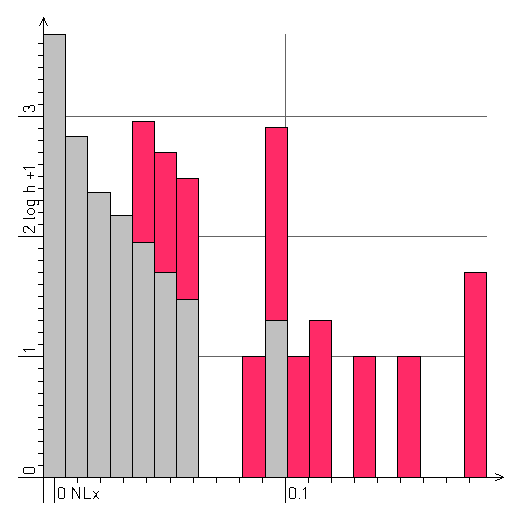
\includegraphics[scale=0.85]{figures/ccc_son}
  }
  \subfigure[tme-Merkmale]{
    \includegraphics[scale=0.85]{figures/ccc_tme}
  }
  \caption{Referenzergenis CCC-Klassifikator (\texttt{common/log/ccc-\_assses-hist\_OK.dn3})}
  \label{fig:ccc}
\end{center}
\end{figure}

\subsection{HMM-Erkenner}

Die erwarteten Ergebnisse befinden sich in den folgenden Dateien:

\begin{tabular}{llll}\toprule
  Typ & Merkmal-Quelle & Verzeichnis\\\midrule
  HMM & tme            & \texttt{[\ldots]/FEAFUS/log.tme/hmm-*.dn3} \\
  HMM & son            & \texttt{[\ldots]/FEAFUS/log.son/hmm-*.dn3} \\
\bottomrule\end{tabular}

% print to ps-file (75x75 mm, DIN-Regular, 8 pt)
% @eakss1
%   find . -name "*.ps" -exec ps2epsi {} \;
%   mmv "*.epsi" '#1.eps'
%   rm *.ps
\begin{figure}[h]
\begin{center}
  \subfigure[son-Merkmale]{
    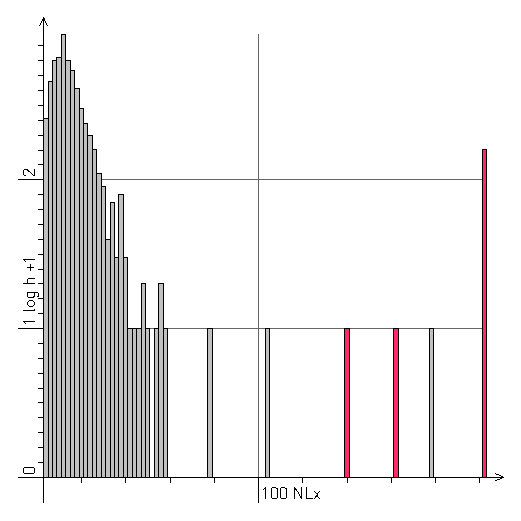
\includegraphics[scale=0.85]{figures/hmm_son}
  }
  \subfigure[tme-Merkmale]{
    \includegraphics[scale=0.85]{figures/hmm_tme}
  }
  \caption{Referenzergenis HMM-Klassifikator (\texttt{FEAFUS/log/hmm-2\_4\_assses-hist\_OK.dn3})}
  \label{fig:ccc}
\end{center}
\end{figure}

\subsection{SVM-Erkenner}

Die erwarteten Ergebnisse befinden sich in den folgenden Dateien:

\begin{tabular}{llll}\toprule
  Typ & Merkmal-Quelle & Verzeichnis\\\midrule
  SVM & tme            & \texttt{[\ldots]/FEAFUS/log.tme/svm-*.dn3} \\
  SVM & son            & \texttt{[\ldots]/FEAFUS/log.son/svm-*.dn3} \\
\bottomrule\end{tabular}

% print to ps-file (75x75 mm, DIN-Regular, 8 pt)
% @eakss1
%   find . -name "*.ps" -exec ps2epsi {} \;
%   mmv "*.epsi" '#1.eps'
%   rm *.ps
\begin{figure}[h]
\begin{center}
  \subfigure[son-Merkmale]{
    \includegraphics[scale=0.85]{figures/svm_son}
  }
  \subfigure[tme-Merkmale]{
    \includegraphics[scale=0.85]{figures/svm_tme}
  }
  \caption{Referenzergenis SVM-Klassifikator (\texttt{FEAFUS/log/svm-\_assses-hist\_OK.dn3})}
  \label{fig:ccc}
\end{center}
\end{figure}

\chapter{Listings}
\section{UASR-Anpassungsskripts}
\subsection{[\ldots]/common/info/cwt1937.itp}
\lstinputlisting[frame=tlbr,basicstyle=\tiny\ttfamily]{cwt1937.itp}

\section{Definitionsdateien}
\subsection{[\ldots]/common/info/classes.txt}
\lstinputlisting[frame=tlbr,basicstyle=\tiny\ttfamily]{classes.txt}
\subsection{[\ldots]/common/info/sensors.txt}
\lstinputlisting[frame=tlbr,basicstyle=\tiny\ttfamily]{sensors.txt}
\subsection{[\ldots]/FEAFUS/info/classes.txt}
\lstinputlisting[frame=tlbr,basicstyle=\tiny\ttfamily]{../../FEAFUS/info/classes.txt}

\section{Konfigurationsdateien}
\subsection{[\ldots]/common/info/feaana.cfg}
\lstinputlisting[frame=tlbr,basicstyle=\tiny\ttfamily]{feaana.cfg}
\subsection{[\ldots]/common/info/feaimp.cfg}
\lstinputlisting[frame=tlbr,basicstyle=\tiny\ttfamily]{feaimp.cfg}
\subsection{[\ldots]/common/info/ccc.cfg}
\lstinputlisting[frame=tlbr,basicstyle=\tiny\ttfamily]{ccc.cfg}
\subsection{[\ldots]/FEAFUS/info/hmm.cfg}
\lstinputlisting[frame=tlbr,basicstyle=\tiny\ttfamily]{../../FEAFUS/info/hmm.cfg}
\subsection{[\ldots]/FEAFUS/info/svm.cfg}
\lstinputlisting[frame=tlbr,basicstyle=\tiny\ttfamily]{../../FEAFUS/info/svm.cfg}

\section{Dateilisten}
\subsection{[\ldots]/common/flists/all.flst}
\lstinputlisting[frame=tlbr,basicstyle=\tiny\ttfamily]{../flists/all.flst}
\subsection{[\ldots]/common/flists/xval.flst}
\lstinputlisting[frame=tlbr,basicstyle=\tiny\ttfamily]{../flists/xval.flst}

\end{document}
